\section{Other inhabitants of the flying castle}

The player can talk to the inhabitant of the flying castle to increase the friendship with them, fulfill optional missions and obtain some bonus.

\subsection{Markl}

\begin{minipage}[t]{0.5\textwidth}
He is Howl’s young apprentice. He is 10 years old and he manages Howl's affairs while he is away, dealing with customers in the different towns linked to by the magic door.

He can put on a cloak and take the appearance of a short, old man.

\subsubsection{Bonus}
\begin{itemize}
	\item wisdom
	\item dexterity
\end{itemize}

\end{minipage}%
%
\hfill
\begin{minipage}[t]{0.4\textwidth}
  \begin{figure}[H]
    \hfill
\includegraphics{Images/Characters/markl_portrait}
    \caption{Markl, movie version}
  \end{figure}
\end{minipage}

\subsection{Witch of the Waste}

\begin{minipage}[t]{0.5\textwidth}
She is a very old woman and she was a powerful witch. She has tried to take Howl’s heart, but Sophie persuaded her to return it to him.

Despite her appearance, she knows a lot about magic. Anyway she doesn’t know about djinns and the spirits realm.

\subsubsection{Bonus}
\begin{itemize}
	\item intelligence
	\item charisma
\end{itemize}

\end{minipage}%
%
\hfill
\begin{minipage}[t]{0.4\textwidth}
  \begin{figure}[H]
    \hfill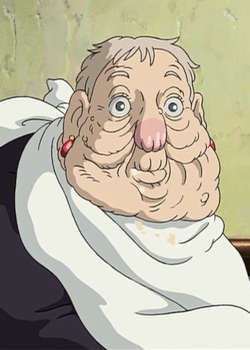
\includegraphics{Images/Characters/witchOfTheWaste_portrait}
    \caption{Witch of the Waste, movie version}
  \end{figure}
\end{minipage}

\subsection{Heen}

\begin{minipage}[t]{0.5\textwidth}
He is a small, furry, old dog. He worked as a spy for Suliman, but then he decided to stay with Sophie and Howl.

He seems always tired but he becomes very worried when Sophie is in danger.

\subsubsection{Bonus}
\begin{itemize}
	\item strength
	\item constitution
\end{itemize}

\end{minipage}%
%
\hfill
\begin{minipage}[t]{0.4\textwidth}
  \begin{figure}[H]
    \hfill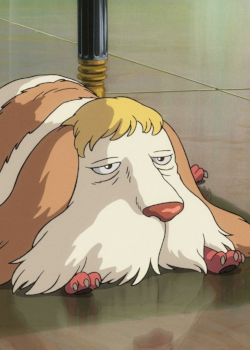
\includegraphics{Images/Characters/heen_portrait}
    \caption{Heen, movie version}
  \end{figure}
\end{minipage}%
%
